\documentclass[hyperref={unicode=true}]{beamer}
%\usepackage{CJKutf8}
\usepackage{multirow}
\usepackage{minted}
\usepackage[slantfont,boldfont]{xeCJK}
\setCJKmainfont{SimSun}
\setCJKmonofont{SimHei}
\usetheme{Darmstadt}
\usecolortheme{beaver}
\input zhwinfonts
\begin{document}
%\begin{CJK}{UTF8}{zhsong}
\setbeamertemplate{caption}[numbered]
\renewcommand\figurename{图}
\renewcommand\tablename{表}
\renewcommand\contentsname{\centering 目录}

%%------------------------------------------
\title{UpBit位图索引的改进}
\subtitle{《软件设计与开发实践》课程答辩}
\author{马玉坤}
\institute{哈尔滨工业大学计算机科学与技术系}
\date{2017年6月15日}
%%------------------------------------------

\begin{frame}
  \titlepage
\end{frame}

\begin{frame}
  \tableofcontents
\end{frame}

%distinct cardinality基数是指某个列可能拥有的不重复数值的个数。

\section{UpBit简介}
\subsection{位图索引}
\begin{frame}\frametitle{位图索引}
  \begin{block}{位图索引 ({\bf Bitmap Index})}
    使用位图来索引数据库信息的数据结构,广泛用于数据库系统中。
  \end{block}
\end{frame}

\begin{frame}\frametitle{位图索引(Cont'd)}
  \begin{table}[H]
    \centering
    \begin{tabular}{|l|l|l|}
      \hline
      姓名 & 性别 & 身高 \\ \hline
      小A & 男   & 167   \\ \hline
      小B & 女   & 165   \\ \hline
      小C & 男   & 180 \\ \hline
    \end{tabular}
    \label{tb:table} \caption{一个普通的数据库中的表}
  \end{table}
  \begin{itemize}[<+->]
  \item 对于“性别”这个属性来说,只有“男”、“女”两种取值。\footnote{根据性染色体判断生理性别,不考虑性染色体异常情况。}\\
  \item 于是,对于”男“、”女“两种取值,我们可以分别获得两个位向量,分别是101和010。\\
  \item 对不同值对应的位向量进行位操作(与、或、异或),可以进行各种各样的复杂的数据库查询。
  \end{itemize}
\end{frame}

\subsection{位图索引的更新}
\begin{frame}\frametitle{位图索引的更新问题}
  \begin{block}{原地更新}
    如果使用传统的原地更新 (In-place),对于每次修改 (例如修改某个人的身高),最坏情况下将需要修改整个位向量,效率较低。\footnote{只考虑使用压缩算法对位图索引进行压缩的情形。}
  \end{block}
\end{frame}

\subsection{UpBit}
\begin{frame}\frametitle{UpBit}
  UpBit对于更新操作的效率极高,这归功于UpBit的两大利器。
  \pause
  \begin{exampleblock}{Update BitVectors}
    由于压缩算法的存在,如果位向量比较简单 (例如1的个数极少),那么修改操作效率就较高。\\
    因此对于每个位向量,定义一个辅助位向量,扮演缓存的角色,用以保存更新内容。当辅助向量较为复杂后,将辅助向量与位向量进行合并。
  \end{exampleblock}
  \pause
  \begin{exampleblock}{Fence Pointers}
    将每个未压缩的位向量进行分块,把每个块的起始位置对应的压缩后的位置保存到一个指针数组中。这些指针就是Fence Pointers。
  \end{exampleblock}
\end{frame}

\begin{frame}\frametitle{UpBit (Cont'd)}
  \begin{figure}[H]
    \begin{center}
      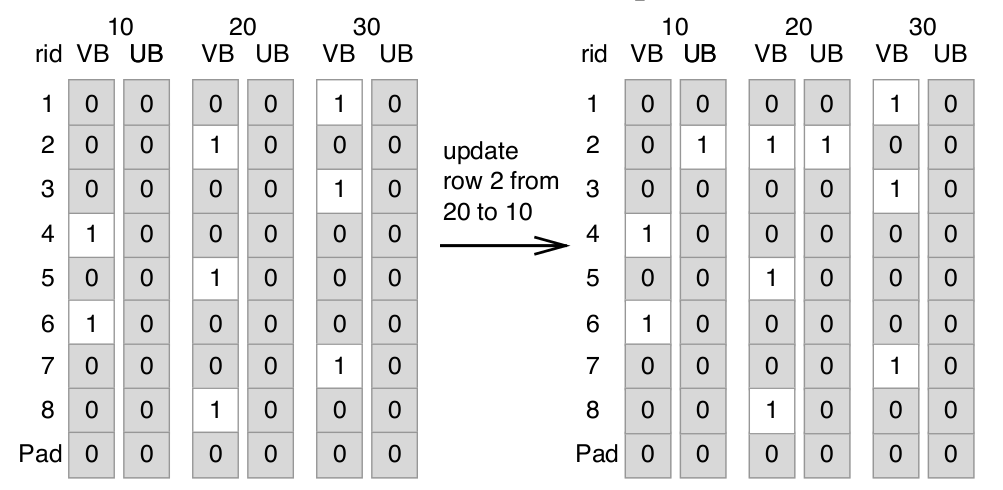
\includegraphics[width=3.5in]{upbit.png}
      \caption{UpBit更新操作}\label{fig:upbit}
    \end{center}
  \end{figure}
\end{frame}

\section{对UpBit的优化}
\subsection{优化动机}
\begin{frame}\frametitle{时间效率}
  \begin{exampleblock}{对行查询}
    \begin{minipage}[c]{0.45\textwidth}
      \begin{itemize}[<+->]
      \item 更新第k行的值,需要找到第k行修改之前的值。
      \item 然而,如图\ref{fig:get_value},寻找第k行的值最坏情况下要遍历所有的位向量。
      \item 实际上,作者实验证明,在基数 ({\bf distinct cardinality})等于1000时,get\_value函数耗时占update总耗时的93\%。
      \end{itemize}
    \end{minipage}
    \begin{minipage}[c]{0.45\textwidth}
      \begin{figure}[H]
        \begin{center}
          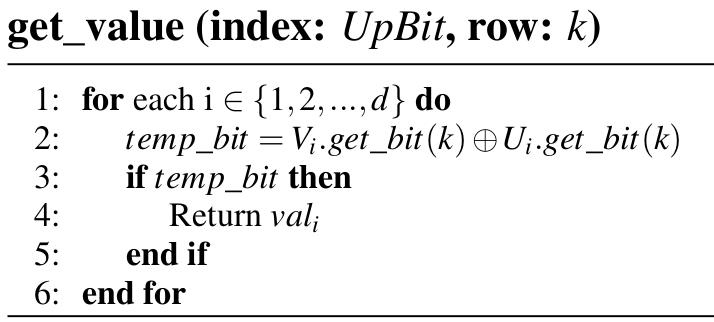
\includegraphics[width=2.1in]{get_value.png}
          \caption{UpBit对行查询}\label{fig:get_value}
        \end{center}
      \end{figure}
    \end{minipage}
  \end{exampleblock}
\end{frame}
\begin{frame}\frametitle{时间效率 (Cont'd)}
  \begin{exampleblock}{范围查询}
    \begin{itemize}[<+->]
    \item 在对数据库查询(例如使用SQL语句)时,我们经常会用到范围查询,比如\mintinline{sql}{SELECT * FROM Persons WHERE Year>1965}。
    \item 然而,直接使用UpBit进行范围查询的效率是较低的。最坏情况下需要遍历所有的位向量。
    \end{itemize}
  \end{exampleblock}
\end{frame}

\begin{frame}\frametitle{空间效率}
  \begin{alertblock}{对Update BitVectors的正确认识}
    \begin{itemize}[<+->]
    \item 实际上,Update BitVectors在UpBit中起了缓存的作用
    \item 在计算机中,缓存的大小是远远小于主存的大小的。
    \item 类比计算机系统中的缓存,实际上不需要在内存中为每个位向量都维护一个Update BitVector。
    \item 甚至可以使用计算机系统中的缓存的替换算法,来有效率地维护Update BitVector。
    \item 这样做不仅可以减小Update BitVectors内存的占用,还不会降低UpBit的性能。
    \end{itemize}
  \end{alertblock}
\end{frame}

\subsection{优化方法}
\begin{frame}\frametitle{对UpBit优化的方法}
  \begin{block}{树状数组 ({\bf Fenwick Tree})}
    \begin{figure}[H]
      \begin{center}
        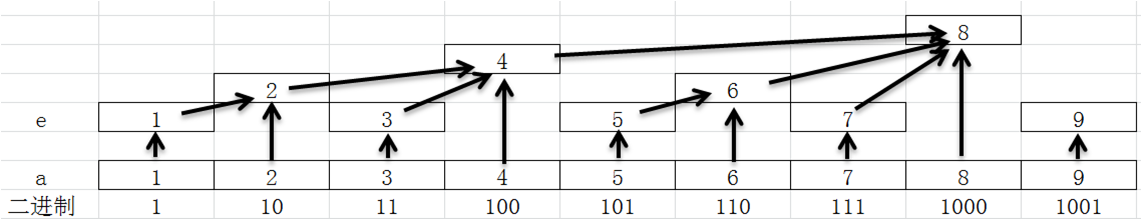
\includegraphics[width=3.5in]{bit.png}
        \caption{树状数组 ({\bf Fenwick Tree})}\label{fig:bit}
      \end{center}
    \end{figure}
    如图\ref{fig:bit},每个节点对应一个位向量,该位向量为对其子节点的位向量进行或操作后的结果。
  \end{block}
\end{frame}
\begin{frame}[fragile]\frametitle{对UpBit优化的方法 (Cont'd)}
  \begin{block}{使用树状数组作为UpBit的组织形式}
    \begin{itemize}
    \item 对行查询:\\
      \begin{enumerate}[1.]
      \item 找到最大的i,使得前i个值的位向量或操作后第k位为0。val[k]即为i+1。
      \item 从值的二进制表示中,由最高位到最低位依次确定。
      \end{enumerate}
    \item 范围查询:\\
      \begin{enumerate}[1.]
      \item 树状数组求前缀和
      \item \begin{minted}{C++}
while (k > 0) {
  res |= val[k];
  k -= lowbit(k);
}
      \end{minted}
      \end{enumerate}
    \end{itemize}
  \end{block}
\end{frame}

\subsection{实验结果}
\begin{frame}\frametitle{对行查询的效率}
  \begin{figure}[H]
    \begin{center}
      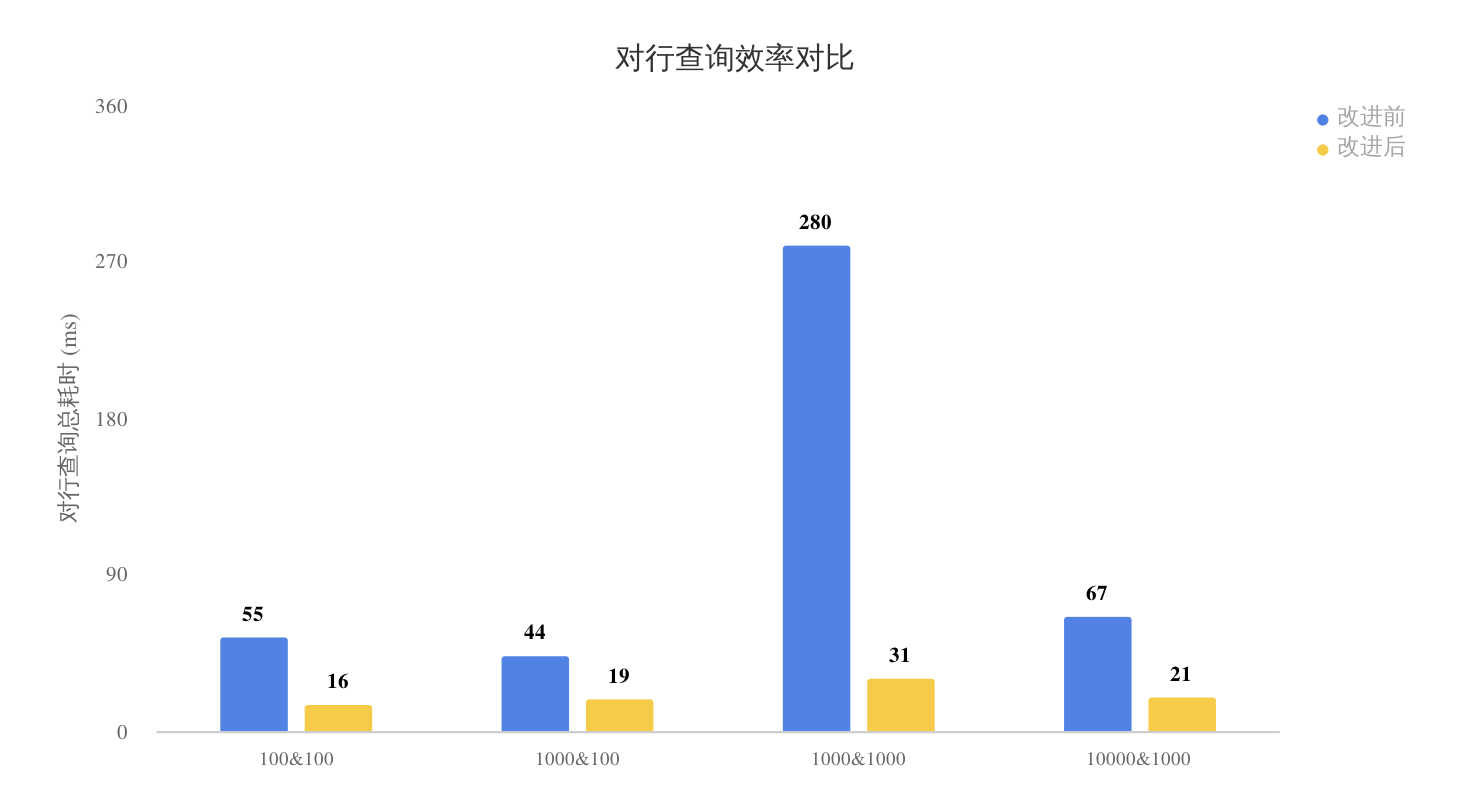
\includegraphics[width=4.5in]{row.png}
      \caption{对行查询效率比较图}\label{fig:row}
    \end{center}
  \end{figure}
\end{frame}
\begin{frame}\frametitle{范围查询的效率}
  \begin{figure}[H]
    \begin{center}
      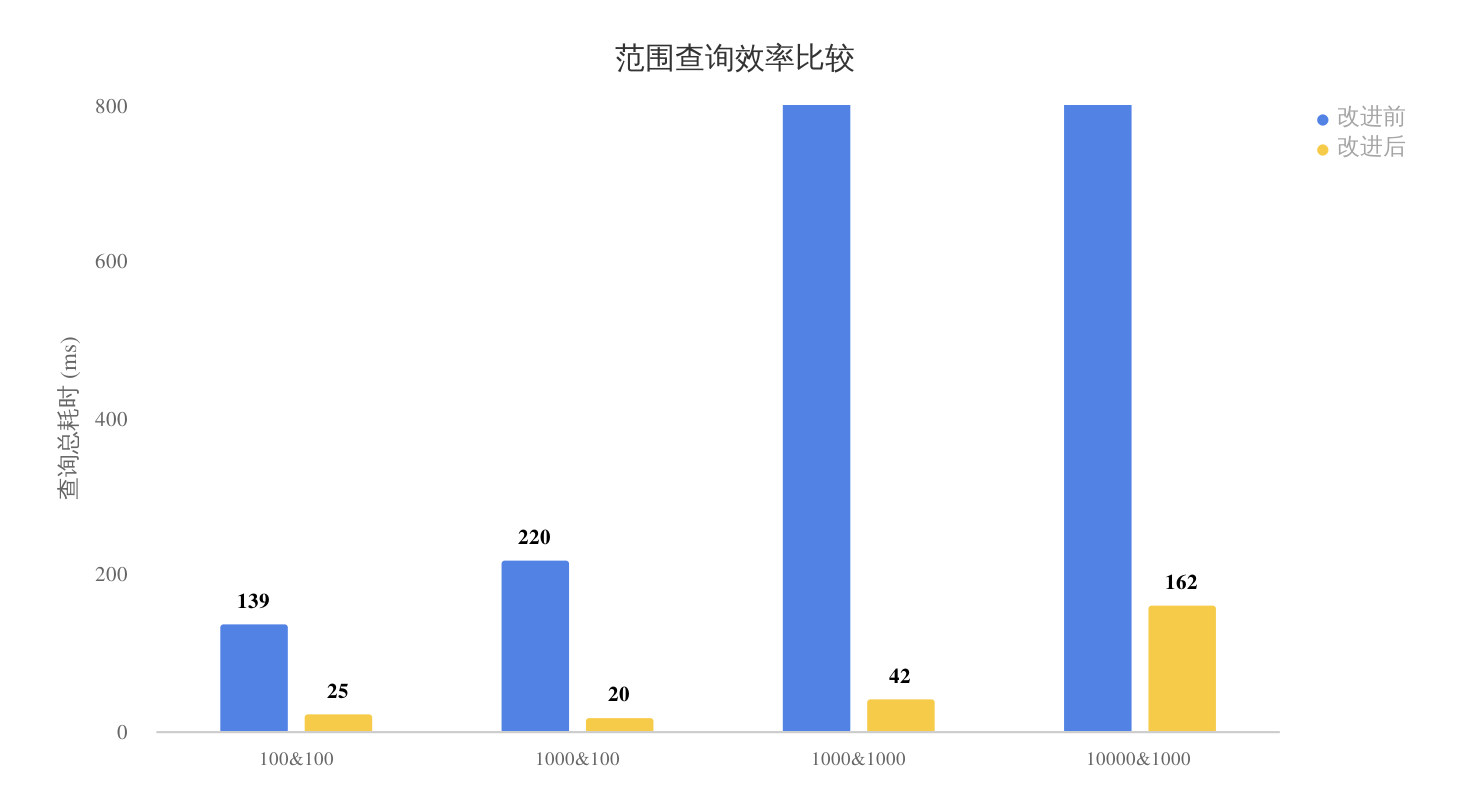
\includegraphics[width=4.5in]{query.png}
      \caption{范围查询效率比较图}\label{fig:query}
    \end{center}
  \end{figure}
\end{frame}
\begin{frame}\frametitle{单值修改的效率}
  \begin{figure}[H]
    \begin{center}
      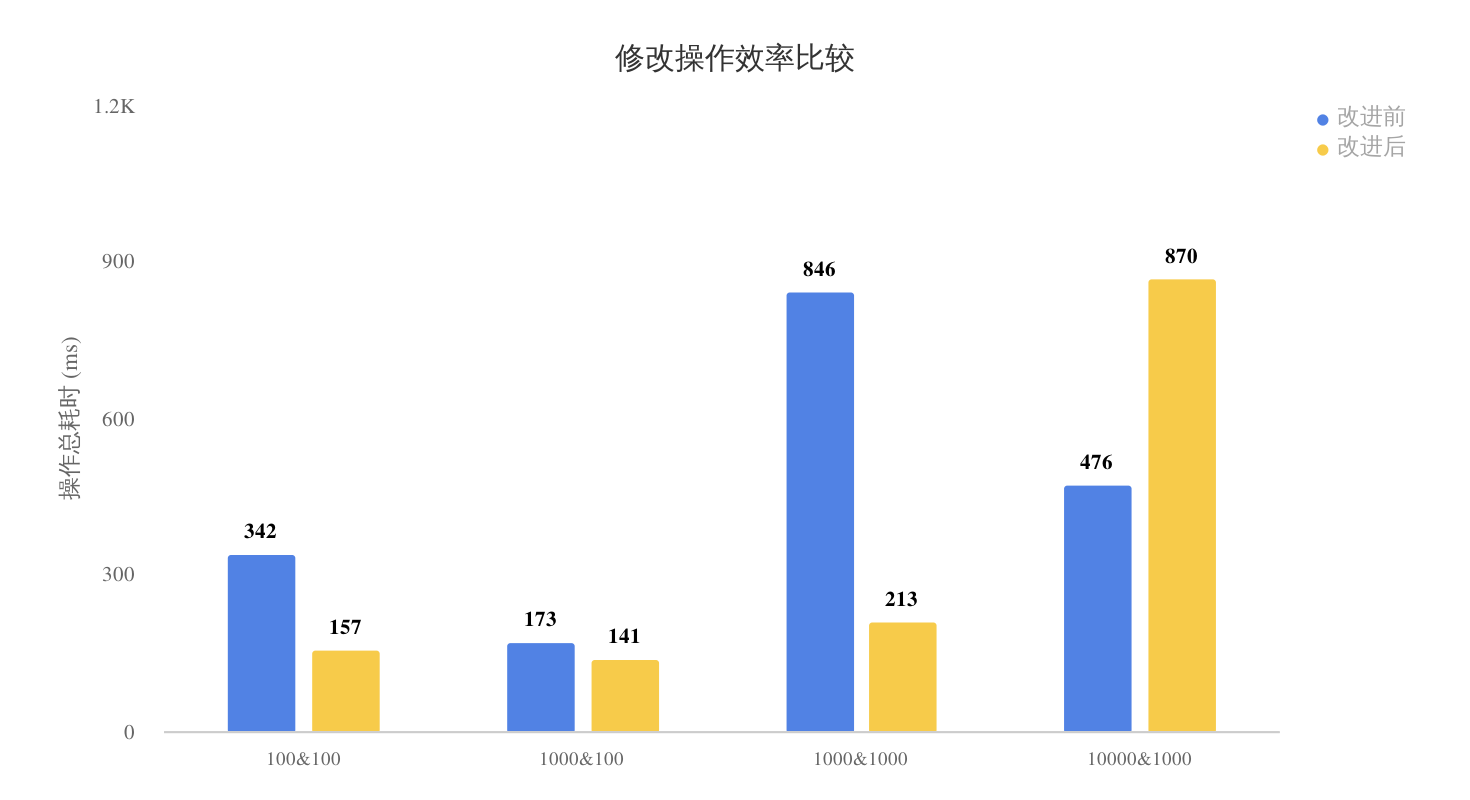
\includegraphics[width=4.5in]{update.png}
      \caption{修改操作效率比较图}\label{fig:update}
    \end{center}
  \end{figure}
\end{frame}

\section{结论}
\begin{frame}\frametitle{结论}
  基于上述研究,我们可以得出以下结论:
  \begin{itemize}[<+->]
  \item 改进后的UpBit对于范围查询效率更高
  \item 改进后的UpBit在基数较大的情况下修改操作效率更高
  \item 改进前的UpBit在基数较小的情况下修改操作效率较高
  \item 如果将树状数组修改为其他平衡树(例如Splay),将能够在取值集合未知的情况下,动态向属性的取值集合添加元素。(尽管效率可能下降。)
  \item 高效地利用Update BitVector将能在不影响效率的情况下减少其内存使用。
  \end{itemize}
\end{frame}

\end{document}
